% EA
\subsubsection{Evolutionary Algorithms} \label{s:lit:ea_overview}

% In the previous section described how graphs are used to analyse the gene interactions and a similar approach but the different algorithm is \acrfull{cgp}. This is part of the \acrfull{ea} family which draws inspiration from the Darwinian evolution.

\begin{figure}[!htb]
  \centering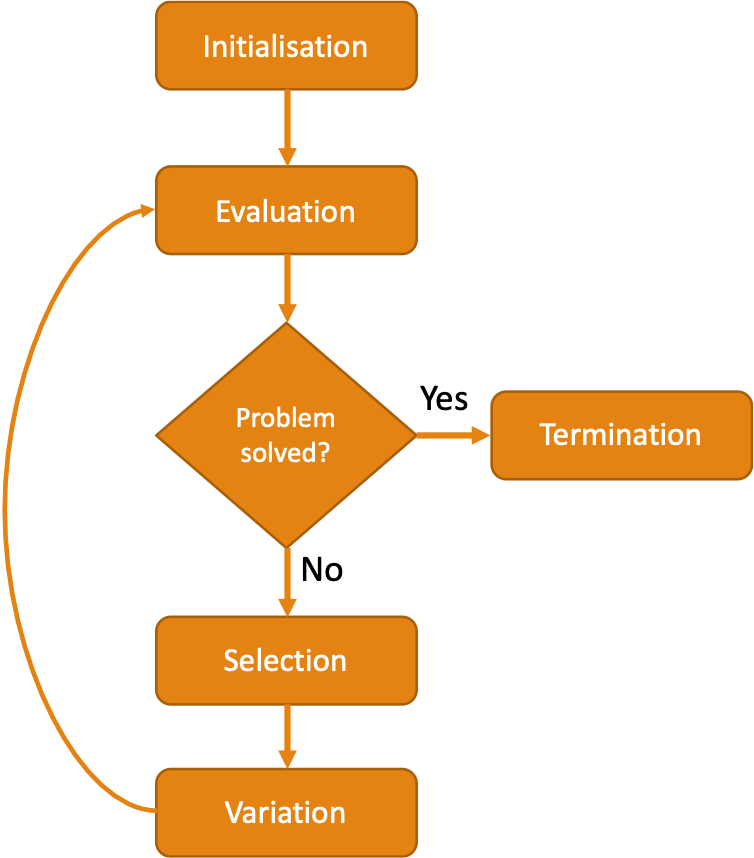
\includegraphics[width=0.4\textwidth,height=0.4\textheight,keepaspectratio]{Images/Resources/EA_basic.png}
    \caption{Evolutionary Algorithms algorithm.}
    \label{fig:ea_basic}
\end{figure}
\FloatBarrier


\acrlong{ea} are a type of \acrshort{ml} that draws inspiration from Darwinian evolution. By incorporating random changes in the algorithm, EA can be used for optimisation or search problems. Thus, EAs are suitable for doing a wide search of the solution space\footnote{Imagine the solution space as space of the total possible solutions for a problem.} which means that they might find an unusual solution and escape the local minimum. A useful analogy here is to think as one climbing a mountain (search space), the goal (optimal solution) is to reach the highest peak but along the way, there are other peaks (local minimum) but smaller (less optimal) than the highest peak (optimal solution). The process (algorithm) in reaching the desired peak is incremental and it requires choosing the right path to reach the global top. Usually, an algorithm has difficulties in differentiated between the highest peaks and the smaller ones, but due to the high variation characteristic of EA, these methods perform well in such problems.


However, these algorithms have a high computational cost and do not usually scale well, therefore are applied to relatively small problems (i.e. number of features). The corollary is that EAs are easier to understand compared to the  \acrfull{dl} (explored in \cref{s:lit:dl_genomics}) and are classified as a 'white-box' approach. In \cref{s:lit:mutations} is presented the MDPFinder (\citet{Zhao2012-wj}) model where \acrfull{ga}, a simpler version of EAs, are applied to process both Gene Expression and mutations.

% would split the sentence here. You could then link to your next point, perhaps: "...from Darwinian evolution. By incorporating random changes in the parameters of a model, or set of models, EA can be used for optimisation..." Something like this makes it clearer why the Darwinian principles are important

As EA resembles the evolutionary process there is also some shared terminology, an individual in the EA context represents a potential solution and a population is a collection of potential solutions. \Cref{fig:ea_basic} describes the algorithmic flow of the evolutionary approach which starts with the initialisation stage, where the individuals are given (usually) random values, followed by the second stage where the fitness of the individuals is measured; i.e. how suitable they are for the problem. If the problem is not solved, then select only the fittest individuals which are then mutated/crossover, introducing variation to the new population. Like in biology, this last step, gives EA a large variety of individuals. This set of steps is run until an individual fits the solution/problem. It is worth mentioning, that the mutation rate, crossover and how the individual is selected, are preset parameters. 


Defining the fitness function as well as encoding the data for the EA algorithm is one of the challenges when developing EA as it is problem specific. Biological evolution is a process that takes time and many iterations, the in-silico adaptation share that and it is the reason for not scaling well or as it has a high computational cost.

The MDPFinder model presented in \cref{s:lit:mutations} used a variation of EA, called \acrfull{ga} which is a simpler version of the EA family where individuals resemble the chromosome. \acrfull{cgp} is another EA algorithm which it's used to process graph representation and it overcomes some of the limitations of the simpler EA methods. As we've seen that graph representation it's already been used in gene networks, CGP may represent an interesting venue to follow. 




% ANN
\subsubsection{Artificial Neural Networks} \label{s:lit:ann_overview}


\begin{figure}[!htb]
\centering
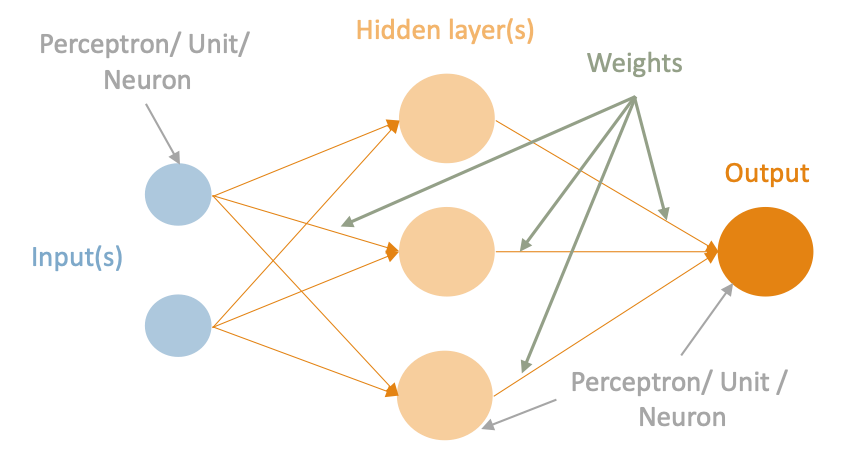
\includegraphics[width=0.7\textwidth,height=0.7\textheight,keepaspectratio]{Images/ANN/Basic_ANN.png}
    \caption{A Simple ANN architecture. }
    \label{fig:ann_basic}
\end{figure}
\FloatBarrier

As it was mentioned at the beginning of this chapter, the connectionist approach is what drives the current AI hype and it's due to the advances in both algorithms and computational power. The inspiration comes from how the brain draws the information from the external stimuli, stores it in memory and retrieve it. Despite being many unknowns to the brain, the main components that are involved in the learning process are the neurons and the synapses between them\footnote{The neurons and synapses are the main components, but there may be others like dendrites which can also be computational units as seen later in the section.}. The simplest learning rule was introduced by Donald Hebb which states "Neurons that fire together, wire together"\cite{Hebb_Donald1949-nn}. This means that a neuron that fire or its concurrently activated with another one (or in a given time window) the two form a stronger connection. The opposite is true, the synapse is weaken, when two neurons that do not get activated in the same time window.

\Cref{fig:ann_basic} it's a simple, single-layer, feed-forward Neural Network where a layer represents a collection of units that usually have the same activation function. In the case of \acrfull{dnn}, the ANN is constructed by many such layers with a large number of units. The neurons are the computational component, each having an activation function that 'tells' the unit when to activate and send a signal across the synapse. The connections between the units are assigned a weight that gives the strength of the synapses. The information is stored in the connections between the units, and it follows Donald Hebb's learning rule stated earlier. Therefore, the central goal of ANN is to find the specific combination of weight values that gives the desired output. Previously, we mentioned different types of learning, in the supervised case, there is an algorithm that has been the engine of the connectionist approach, called back-propagation. As the name suggests, this method propagates the input's error from the output layer back, this information is used then to compute new values for the network's weights; this is called stochastic gradient descent.
%  This algorithm is not used in the biological NN and it relies on the data given and may inherit its biasis\footnote{For example the data is collected only for a specific demographic.}. 


\paragraph*{Autoencoders} \label{s:lit:autoencod_overview}

Autoencoders are a particular type of Deep Neural Networks and \cref{fig:autoencoders} represents a diagram a simple Autoencoder architecture in which it can be seen that there are 3 main components. The input layer to which the data is fed, for more complex models it has additional hidden layers and with the input, the two layers are known together as the encoder stage. The bottleneck part is where the data is compressed into a lower dimension. Next, a mirror to the encoder, the decoder, is dealing with reconstructing the outputs of the bottleneck into original data; hence, the name. This part of autoencoders is an advantage over the PCA as the original data can be reconstructed from the lower dimension. A derivative of Neural Networks, autoencoders are more suitable to find non-linear patterns in the data as whereas PCA finds only linear patterns. With all these advantages as dimension reduction techniques is not a surprise that there has been some work on applying Autoencoders to genomics (explored further in \cref{s:lit:autoencoders}).

Autoencoders are the most successful \acrshort{dnn} approaches to genomics problems where they have been used as a dimension reduction technique to solve the dimension curse of genetic data, where few samples are available with a large number of features (genes). This means, that they are not replacing the clustering models but techniques like \acrfull{pca} or \acrfull{nmf}, and will be used in conjunction with clustering techniques.

\begin{figure}[!htb]
\centering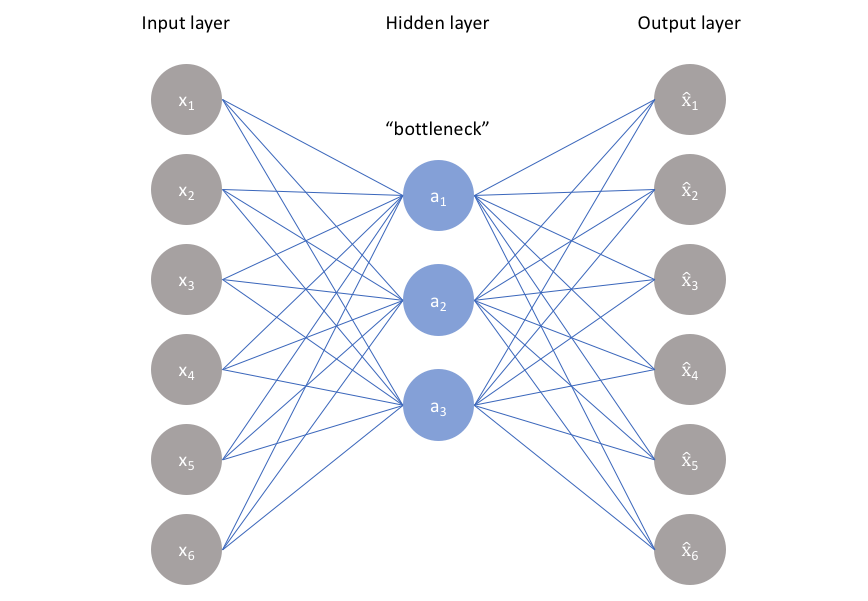
\includegraphics[width=0.8\textwidth,height=0.5\textheight,keepaspectratio]{Images/Autoencoders/simple_autoencoders.png}
    \caption{Simple architecture of autoencoders, from \cite{Jordan2018-bc}}
    \label{fig:autoencoders}
\end{figure}
\FloatBarrier

\subsubsection{Deep Learning  and Genomics} \label{s:lit:dl_genomics}

\vspace{3mm}
\fbox {
    \parbox{\linewidth}{
      \begin{itemize}
        \item Autoencoders used with other methods to predict patient survival 
        \item Autoencoders seems to preserve biological data better than other dimension reduction techniques
        \item Other deep learning has limited applications to genomics
      \end{itemize}
    }
}
\vspace{3mm}

Deep Learning has been the steam engine that fueled the recent progress in Machine Learning, but usually, these models are applied to supervised learning problems and require a large number of samples. In comparison, defining better bladder cancer subtypes from the Gene Expression, mutations \& other data is an unsupervised learning problem. On top of that, the current sequencing technologies are not affordable enough to enable large datasets. This means, that, currently, most of the \acrshort{dl} approaches are not (yet) suitable to the specific multi-omics problem except the Autoencoders.

The above statement is further supported by a review paper on "The Application of Deep Learning in Cancer Prognosis" by \citet{Zhu2020-cv}, where on the multi-omics section, no 'traditional' \acrshort{dl} are used except for the Autoencoders. Furthermore, the authors provide suggestions to overcome the limitations of \acrshort{dnn} to the cancer research. The ones relevant to this PhD project are data augmentation or imputation, building the models using more domain knowledge, and the use of one-shot techniques. The first suggestion is already been adopted in the field where many researchers have created synthetic data \cite{Zhao2012-wj,Leiserson2015-yk} following the distributions from realistic datasets. Next, this PhD project benefits of domain knowledge by being supervised by members of the Jack Birch Unit (JBU), which has leading expertise in bladder cancer and data on the normal

The last suggestion, One-Shot learning, is intriguing and worth considering but based on the work done by OpenAI it may have some limitations. In their "One-Shot Imitation Learning" paper, \citet{duan2017-ae} are using domain randomisation to train their robot to perform a task (building a tower from different blocks) in a simulated world. The trained model is then used to replicate a similar task in the real-life after a human performed a building task that was not present in the training phase. It is challenging to see how this can be applied to a multi-omics problem, where the domain expertise is relevant. Possibly, some tweaking to GPT-3\cite{Brown2020-wh} model (from the OpenAI) may be something worth exploring, but that's been used to generate text and is focused on Natural Language Processing problems. A remote application might be to generate synthetic data to test the computational model\footnote{At the moment of writing OpenAI hasn't opened their model, but I believe that similar but less complex models are available that might be used to generate synthetic data.}. Despite the unfavourable prospects, this may represent an exciting venue to follow when there is more progress on this type of model.

There have been attempts to use \acrshort{dl} to predict survival from omics data, but with less success. In their model, Cox-nnet \cite{Ching2018-gq}, the authors feed \acrshort{tcga} dataset to an \acrshort{ann} for 10 cancers to predict the survival rate. This achieves reasonable prediction scores but is not significantly better than the canonical methods. Despite not being tested on other datasets, Ching et al. indicate that Networks with more layers come with the risk of overfitting the dataset.  


% Other applications of DL in genomics
Indeed, most of the \acrshort{dl} paradigms are not directly applicable to the multi-omics problem, but there have been efforts in solving other biological problems. Most notably as well as one of the most recent is the AlphaFold model\cite{Jumper2021-du} (DeepMind) which predicts the protein folding based on the protein sequence with the highest accuracy of a computational model. This is a breakthrough in biology as predicting protein folding has been considered a hard problem to solve.


\paragraph*{Autoencoders} \label{s:lit:autoencoders}

\citet{Chaudhary2018-qj} are using Autoencoders to predict the survival of patients from a particular type of liver cancer, hepatocellular carcinoma (HCC). They have used the RNA-seq, methylation and miRNA data from TCGA to find the correlations between the survival and HCC. Their model reduced the number of features to 100 which were later clustered with K-means and used the standard metrics to measure the performance (Silhouette and Calinski - Harabasz criterion). The authors show that the autoencoders have been more successful than the PCA at preserving the relevant information. However, how PCA was applied to multi-omics data has not been described in detail. A criticism of the work of \citet{Chaudhary2018-qj} is that predicting survival rate is not the most informative as it does not help understanding how to improve the current treatment whereas better cancer subtyping does.

Most importantly, Chaudhary confirms that a DL model using multi-omics data yields a better result than one receiving single-omics data. This is further supported by the Tianle Ma and Aidong Zhang work in \cite{Ma2019-hk}. These can only, strengthen the project's hypothesis that adding mutation data, and other available data will yield better predictions.

The work of \citet{Ma2019-hk} is another instance where Autoencoders are applied to TCGA data. More specifically, the authors used Bladder and Brain Lower Grade Glioma (LGG) on gene expression, miRNA, DNA methylation and protein expression to predict survival events and progression-free intervals. They have also integrated domain knowledge through the molecular interaction network from the STRING database. Their model outperforms the traditional methods and approaches of ML in providing clinical information about tumour events.

Autoencoders have been used for processing somatic mutation datasets. In one of the first pieces of work in this realm, Palazzo et al. \cite{Palazzo2019-hx} use AutoEncoders to represent in lower dimension the somatic mutations from 40 different tumour types/subtypes. The authors acknowledged that their results are promising to preserve biological information in lower dimensions but need further validation.

% is is all very interesting! Can you give specifics, particularly on the bladder work in the previous paragraph - what did they specifically improve, do they link to mRNA subtypes at all etc?

All in all, the work done suggest that Autoencoders are a good dimension reduction technique for multi-omics datasets. Their versatility on the input data represents one of the advantages along with reducing nonlinear patterns. In addition, some of the works suggests that Autoencoders preserve biological knowledge, but it needs further validation to support the assumption. It can be seen that Autoencoders were mostly used to predict the survival of a cancer patient and not to refine the cancer subtyping which is more useful to improve the current treatments. Also, multi-omics data was given to the Autoencoders but not Gene Expression with mutations, which we know have a strong biological correlation between tumours.




% Choosing the right ML approach
\subsubsection{Choosing the right ML approach} \label{s:lit:neuroevolution}

\Cref{s:lit:ea_overview} covered the basics of the evolutionary approach, and in both \ref{s:lit:ann_overview} \& \ref{s:lit:autoencod_overview} sections it was presented the connectionists' view of ML. These two solve different types of problems, where so far, the EAs are better for search problems and the ANNs for classification. The ANNs work by finding an optimal configuration of the weights and network topology, which can be seen as a search/optimisation problem for the right network configuration. Therefore, there has been work in combining the two approaches in what is called Neuroevolution. Such an approach has been used to process mutations data and it's covered in \cref{s:lit:mutations}.

In these computational methods, EAs are used to find the optimal initial configuration of the ANN, which then it's used to be trained. Starting from a different than random state helps the ANN to avoid the local minimum problem, and to increase the classifications performances. On top of that, the EAs are also used to determine the best network topology which means the number of layers, units, their connections, etc.

Therefore, choosing the right ML depends on the problem statement as EA and ANN are good in specific situations, but can also be combined to take advantage of both worlds. The next section attempts to cover the work done across the genomics field by looking at various approaches depending on the datasets used.
